% ==========================================
% BAB IV PERANCANGAN
% ==========================================
\cleardoublepage
\chapter{PERANCANGAN}
\label{chap:perancangan}

\section{Gambaran Umum Sistem}

\subsection{Use Case}

Pada sistem aplikasi pembelajaran Algoritma dan Struktur Data berbasis \textit{guided learning} ini, terdapat satu aktor yaitu \textit{user} yang merupakan mahasiswa sebagai pengguna sistem. \textit{User} berinteraksi dengan sistem untuk mempelajari materi ASD secara terstruktur, mulai dari memilih topik, memahami konsep, melihat contoh, mengerjakan latihan, hingga memantau progres belajar.

Sistem dirancang sebagai \textit{teman belajar digital} yang mendampingi mahasiswa dalam proses pembelajaran. Melalui integrasi LLM, sistem mampu memberikan penjelasan materi, contoh implementasi, serta umpan balik terhadap latihan yang dikerjakan oleh \textit{user} secara interaktif dan adaptif.

Berikut merupakan \textit{use case diagram} yang menggambarkan interaksi antara \textit{user} dengan sistem pembelajaran ASD.

\begin{figure}[H]
    \centering
    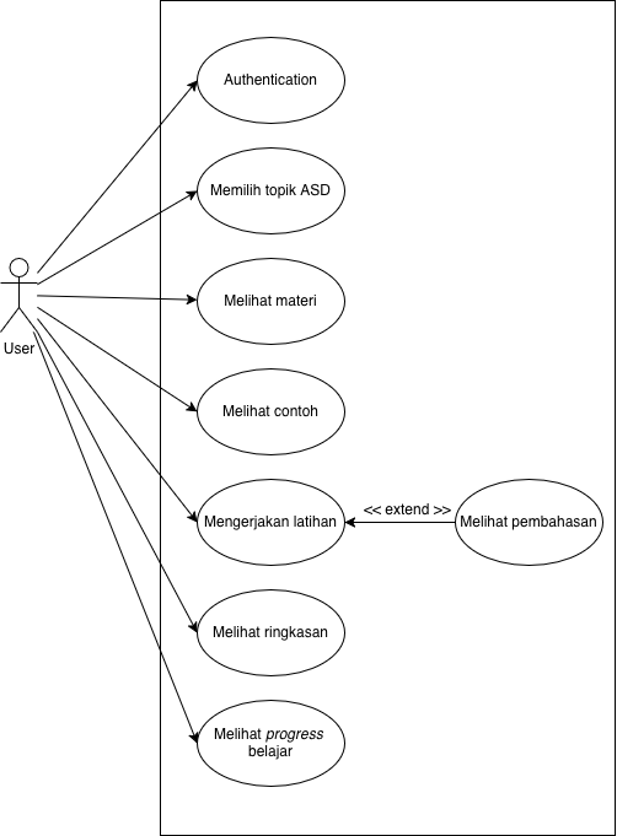
\includegraphics[width=0.75\textwidth]{images/use-case-diagram.png}
    \caption{Diagram \textit{Use Case} Sistem Teman Belajar ASD}
    \label{fig:use-case}
\end{figure}

Penjelasan mengenai diagram di atas dan keterkaitannya dengan kebutuhan fungsional dapat dilihat pada Tabel \ref{tab:use-case}.

\begin{longtable}{|p{1.2cm}|p{1.5cm}|p{2.8cm}|p{5.5cm}|p{1.8cm}|}
\caption{Deskripsi \textit{Use Case} Sistem Pembelajaran ASD}
\label{tab:use-case}\\
\hline
\textbf{ID} & \textbf{Aktor} & \textbf{Use Case} & \textbf{Deskripsi} & \textbf{Functional Requirements} \\
\hline
\endfirsthead

\caption[]{Deskripsi \textit{Use Case} Sistem Pembelajaran ASD (lanjutan)}\\
\hline
\textbf{ID} & \textbf{Aktor} & \textbf{Use Case} & \textbf{Deskripsi} & \textbf{Functional Requirements} \\
\hline
\endhead

\hline
\multicolumn{5}{r}{\textit{Bersambung ke halaman berikutnya}}\\
\endfoot

\hline
\endlastfoot

UC-01 & User & Authentication &
User melakukan \textit{login} dengan memasukkan kredensial berupa \textit{email} dan \textit{password} untuk mengakses sistem pembelajaran. &
FR-01 \\
\hline

UC-02 & User & Memilih topik ASD &
User memilih topik pembelajaran ASD yang ingin dipelajari sebagai langkah awal dalam alur belajar. &
FR-02 \\
\hline

UC-03 & User & Melihat materi &
User menerima penjelasan konsep ASD yang dihasilkan sistem secara terstruktur sesuai topik yang dipilih. &
FR-03 \\
\hline

UC-04 & User & Melihat contoh &
User melihat contoh implementasi atau ilustrasi dari konsep ASD untuk membantu pemahaman. &
FR-04 \\
\hline

UC-05 & User & Mengerjakan latihan &
User mengerjakan soal latihan yang diberikan sistem untuk menguji pemahaman terhadap materi. &
FR-05 \\
\hline

UC-06 & User & Melihat pembahasan &
User melihat pembahasan dari latihan yang telah dikerjakan sebagai bentuk umpan balik dari sistem. Relasi \textit{extend} dari UC-05 menunjukkan bahwa pembahasan hanya tersedia setelah \textit{user} mengerjakan latihan. &
FR-06 \\
\hline

UC-07 & User & Melihat ringkasan &
User melihat rangkuman materi untuk memperkuat pemahaman terhadap konsep yang telah dipelajari. &
FR-07 \\
\hline

UC-08 & User & Melihat \textit{progress} belajar &
User dapat melihat progres pembelajaran yang menunjukkan sejauh mana materi telah dipelajari. &
FR-08 \\
\hline

\end{longtable}

Tabel \ref{tab:use-case} menunjukkan bahwa terdapat satu aktor yaitu \textit{user} yang dapat menjalankan berbagai aktivitas untuk memenuhi kebutuhan fungsional sistem. Proses pembelajaran dimulai dari \textit{user} melakukan autentikasi (UC-01), kemudian memilih topik ASD yang ingin dipelajari (UC-02).

Selanjutnya, \textit{user} akan memasuki alur pembelajaran terstruktur dengan melihat materi (UC-03) yang berisi penjelasan konsep yang dihasilkan sistem. Untuk memperdalam pemahaman, \textit{user} dapat melihat contoh implementasi (UC-04) sebelum mengerjakan latihan yang diberikan (UC-05).

Setelah menyelesaikan latihan, \textit{user} dapat melihat pembahasan (UC-06) sebagai bentuk umpan balik dari sistem. Relasi \textit{extend} antara UC-05 dan UC-06 menunjukkan bahwa pembahasan hanya muncul setelah \textit{user} mengerjakan latihan. Selain itu, \textit{user} juga dapat melihat ringkasan materi (UC-07) untuk memperkuat pemahaman, serta memantau progres belajar melalui fitur \textit{progress} (UC-08).

Dengan demikian, seluruh \textit{use case} yang dirancang telah mencerminkan alur \textit{guided learning} yang mendukung pembelajaran ASD secara terstruktur dan interaktif, serta memenuhi kebutuhan fungsional sistem.


\subsection{Sequence Diagram}

\textit{Sequence diagram} menggambarkan urutan interaksi antar komponen sistem, \textit{User}, \textit{Frontend}, \textit{Backend}, \textit{Database}, dan OpenAI API, dalam menyelesaikan setiap fungsionalitas. Diagram berikut disusun berdasarkan alur \textit{guided learning} yang telah dirancang, mulai dari autentikasi hingga pemantauan progres belajar.

\begin{figure}[H]
    \centering
    \textbf{FT-01 Login}\\[6pt]
    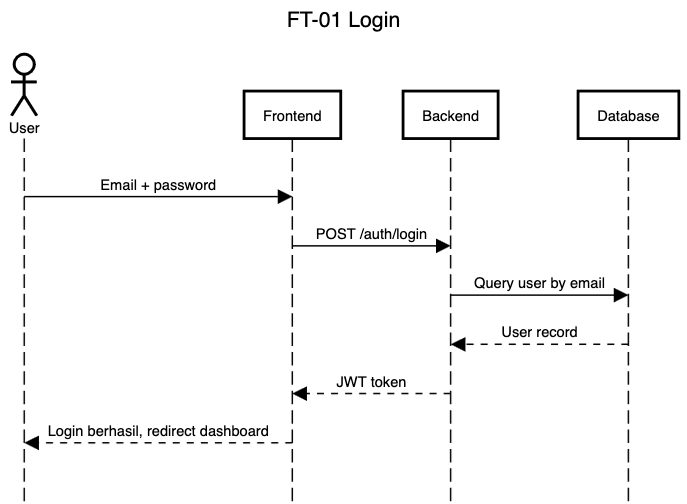
\includegraphics[width=0.9\textwidth]{images/FT-01-Login.png}
    \caption{\textit{Sequence Diagram} FT-01 Login}
    \label{fig:sd-login}
\end{figure}

Diagram pada Gambar \ref{fig:sd-login} menggambarkan alur autentikasi pengguna. \textit{User} memasukkan \textit{email} dan \textit{password} pada \textit{frontend}, yang kemudian mengirimkan permintaan \texttt{POST /auth/login} ke \textit{backend}. \textit{Backend} melakukan \textit{query} data pengguna ke \textit{database} berdasarkan \textit{email} yang diberikan. Jika data ditemukan dan kredensial valid, \textit{backend} mengembalikan JWT \textit{token} ke \textit{frontend}, yang selanjutnya menyimpan \textit{token} tersebut dan mengarahkan \textit{user} ke halaman \textit{dashboard}.

\begin{figure}[H]
    \centering
    \textbf{FT-02 Logout}\\[6pt]
    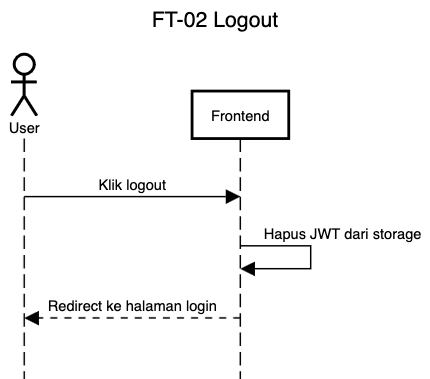
\includegraphics[width=0.55\textwidth]{images/FT-02-Logout.png}
    \caption{\textit{Sequence Diagram} FT-02 Logout}
    \label{fig:sd-logout}
\end{figure}

Diagram pada Gambar \ref{fig:sd-logout} menggambarkan alur keluar dari sistem. Ketika \textit{user} mengeklik tombol \textit{logout}, \textit{frontend} langsung menghapus JWT \textit{token} dari \textit{storage} lokal tanpa perlu melakukan panggilan ke \textit{backend}. Setelah \textit{token} dihapus, \textit{frontend} mengarahkan \textit{user} kembali ke halaman \textit{login}.

\begin{figure}[H]
    \centering
    \textbf{FT-03 Pilih Topik ASD + FT-11 \textit{Guided Learning Flow}}\\[6pt]
    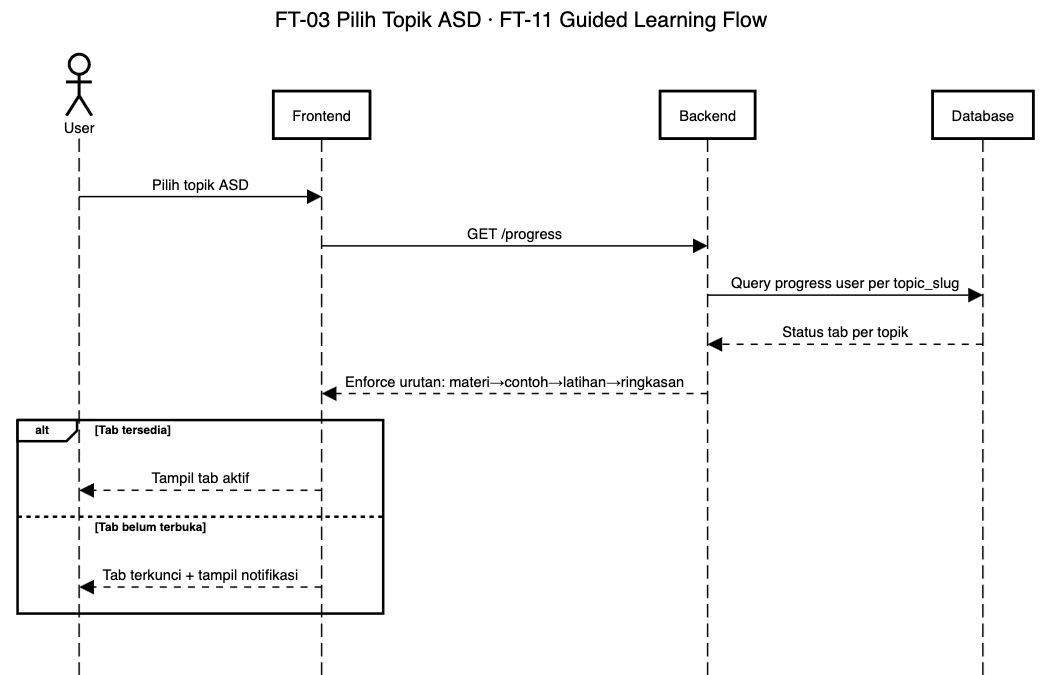
\includegraphics[width=0.9\textwidth]{images/FT-03-Pilih-Topik-ASD-FT-11-Guided-Learning-Flow.png}
    \caption{\textit{Sequence Diagram} FT-03 Pilih Topik ASD dan FT-11 \textit{Guided Learning Flow}}
    \label{fig:sd-pilih-topik}
\end{figure}

Diagram pada Gambar \ref{fig:sd-pilih-topik} menggambarkan alur pemilihan topik ASD sekaligus penegakan urutan \textit{guided learning}. Setelah \textit{user} memilih topik, \textit{frontend} meminta data progres melalui \texttt{GET /progress}. \textit{Backend} mengambil status tab tiap topik dari \textit{database}, lalu menegakkan urutan pembelajaran: materi $\rightarrow$ contoh $\rightarrow$ latihan $\rightarrow$ ringkasan. Jika tab yang ingin diakses sudah tersedia, sistem menampilkan tab tersebut; jika belum terbuka, sistem menguncinya dan menampilkan notifikasi kepada \textit{user}.

\begin{figure}[H]
    \centering
    \textbf{FT-04 Tampilkan Materi + FT-10 \textit{Generate} LLM + FT-14 Adaptasi Konten}\\[6pt]
    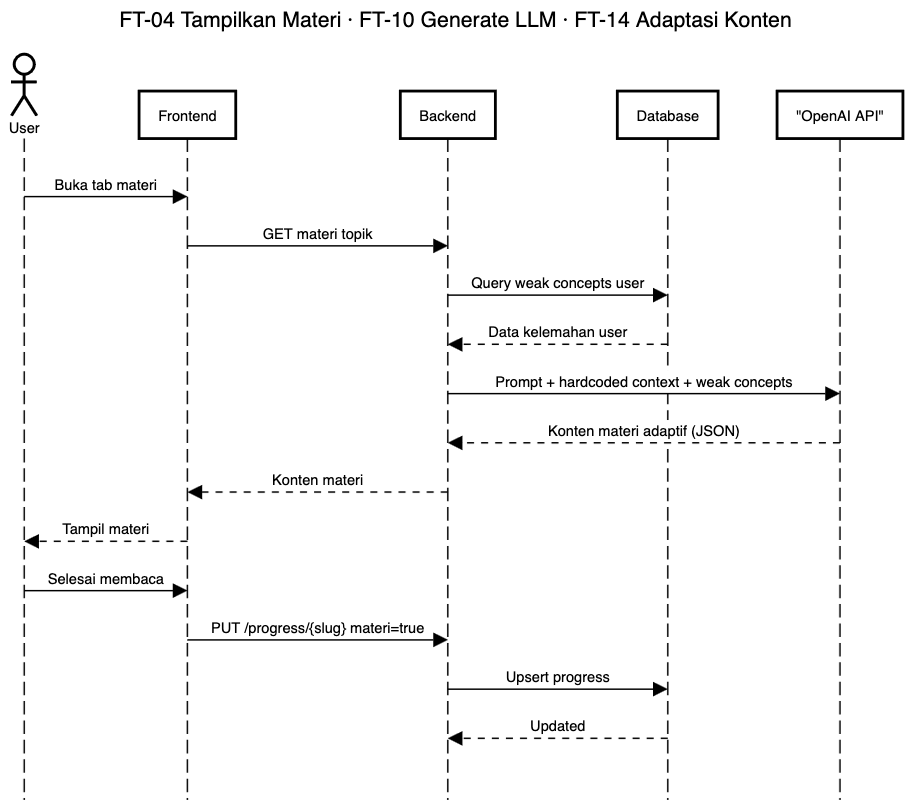
\includegraphics[width=0.9\textwidth]{images/FT-04-Tampilkan-Materi-FT-10-Generate-LLM-FT-14-Adaptasi-Konten.png}
    \caption{\textit{Sequence Diagram} FT-04 Tampilkan Materi, FT-10 \textit{Generate} LLM, dan FT-14 Adaptasi Konten}
    \label{fig:sd-materi}
\end{figure}

Diagram pada Gambar \ref{fig:sd-materi} menggambarkan alur penampilan materi yang dihasilkan LLM secara adaptif. Ketika \textit{user} membuka tab materi, \textit{frontend} mengirim permintaan ke \textit{backend}. \textit{Backend} terlebih dahulu mengambil data kelemahan konsep \textit{user} (\textit{weak concepts}) dari \textit{database}, kemudian menyusun \textit{prompt} yang menggabungkan konteks materi (\textit{hardcoded context}) dan data kelemahan tersebut sebelum dikirim ke OpenAI API. Respons berupa konten materi adaptif dalam format JSON dikembalikan ke \textit{frontend} dan ditampilkan kepada \textit{user}. Setelah \textit{user} selesai membaca, \textit{frontend} memperbarui progres melalui \texttt{PUT /progress/\{slug\}} dengan status \texttt{materi=true}.

\begin{figure}[H]
    \centering
    \textbf{FT-05 Tampilkan Contoh + FT-10 \textit{Generate} LLM + FT-14 Adaptasi Konten}\\[6pt]
    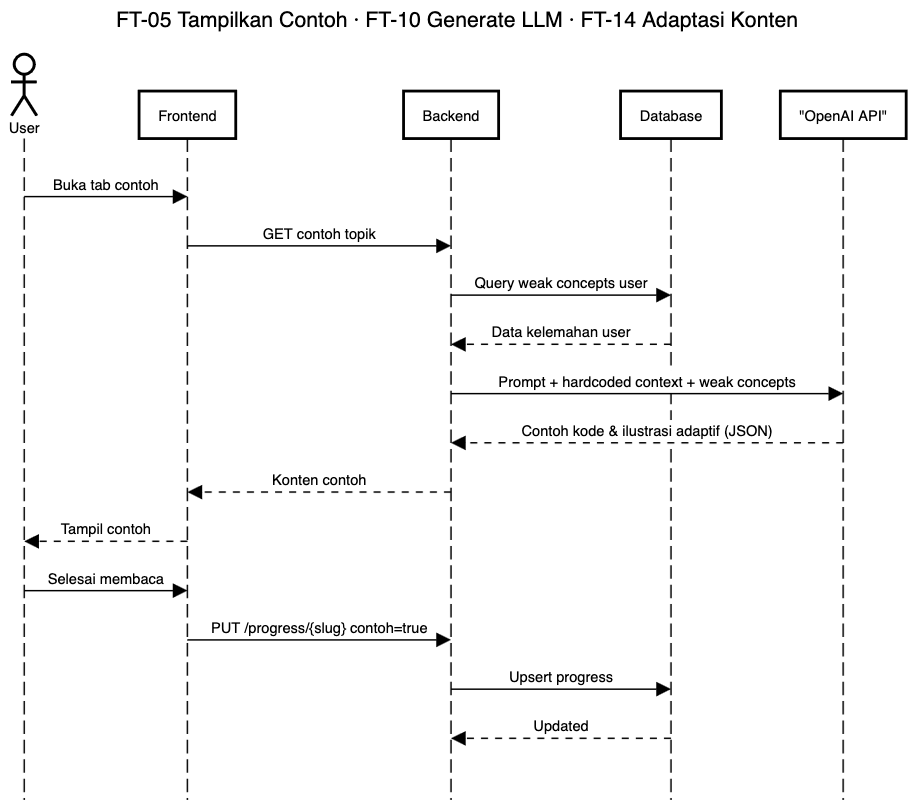
\includegraphics[width=0.9\textwidth]{images/FT-05-Tampilkan-Contoh-FT-10-Generate-LLM-FT-14-Adaptasi-Konten.png}
    \caption{\textit{Sequence Diagram} FT-05 Tampilkan Contoh, FT-10 \textit{Generate} LLM, dan FT-14 Adaptasi Konten}
    \label{fig:sd-contoh}
\end{figure}

Diagram pada Gambar \ref{fig:sd-contoh} menggambarkan alur penampilan contoh implementasi yang bersifat adaptif. Alur ini serupa dengan FT-04, namun keluaran yang dihasilkan OpenAI API berupa contoh kode dan ilustrasi langkah demi langkah yang disesuaikan dengan kelemahan konsep \textit{user}. Setelah \textit{user} selesai mempelajari contoh, progres diperbarui dengan status \texttt{contoh=true} sehingga tab latihan dapat dibuka.

\begin{figure}[H]
    \centering
    \textbf{FT-06 Latihan Soal + FT-10 \textit{Generate} LLM + FT-13 \textit{Adaptive Engine} + FT-14 Adaptasi Konten}\\[6pt]
    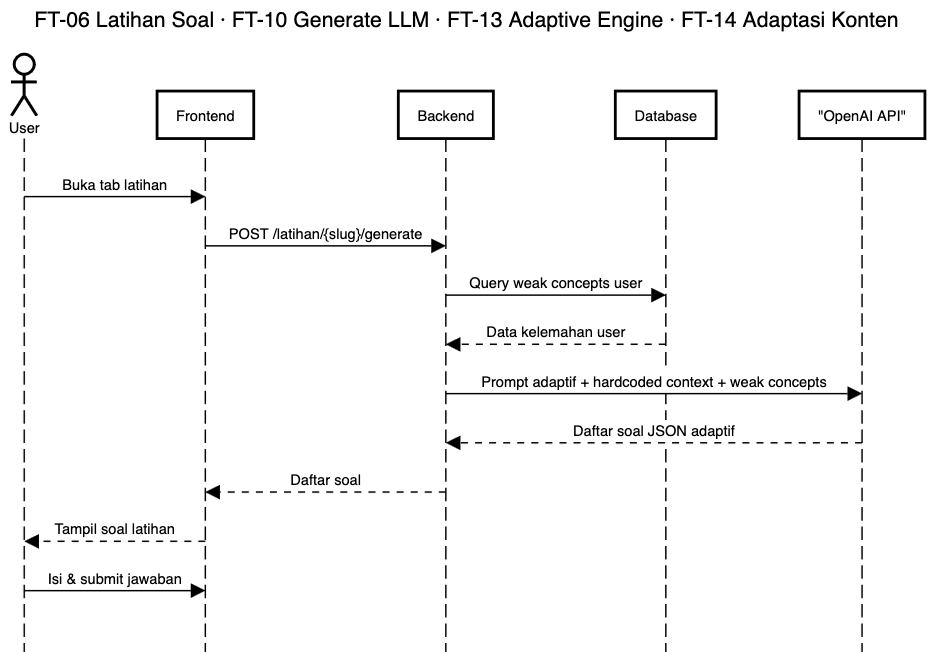
\includegraphics[width=0.9\textwidth]{images/FT-06-Latihan-Soal-FT-10-Generate-LLM-FT-13-Adaptive-Engine-FT-14-Adaptasi-Konten.png}
    \caption{\textit{Sequence Diagram} FT-06 Latihan Soal, FT-10 \textit{Generate} LLM, FT-13 \textit{Adaptive Engine}, dan FT-14 Adaptasi Konten}
    \label{fig:sd-latihan}
\end{figure}

Diagram pada Gambar \ref{fig:sd-latihan} menggambarkan alur pembuatan dan penyajian latihan soal secara adaptif. \textit{Frontend} mengirim permintaan \texttt{POST /latihan/\{slug\}/generate} ke \textit{backend}. \textit{Backend} mengambil data \textit{weak concepts} dari \textit{database} dan menyusun \textit{prompt} adaptif yang memprioritaskan konsep-konsep yang masih lemah bagi \textit{user}. OpenAI API menghasilkan daftar soal dalam format JSON yang kemudian ditampilkan kepada \textit{user}. \textit{User} mengisi jawaban dan melakukan \textit{submit} untuk dievaluasi pada tahap berikutnya.

\begin{figure}[H]
    \centering
    \textbf{FT-07 Pembahasan Latihan + FT-12 \textit{Feedback} Jawaban + FT-13 \textit{Adaptive Engine}}\\[6pt]
    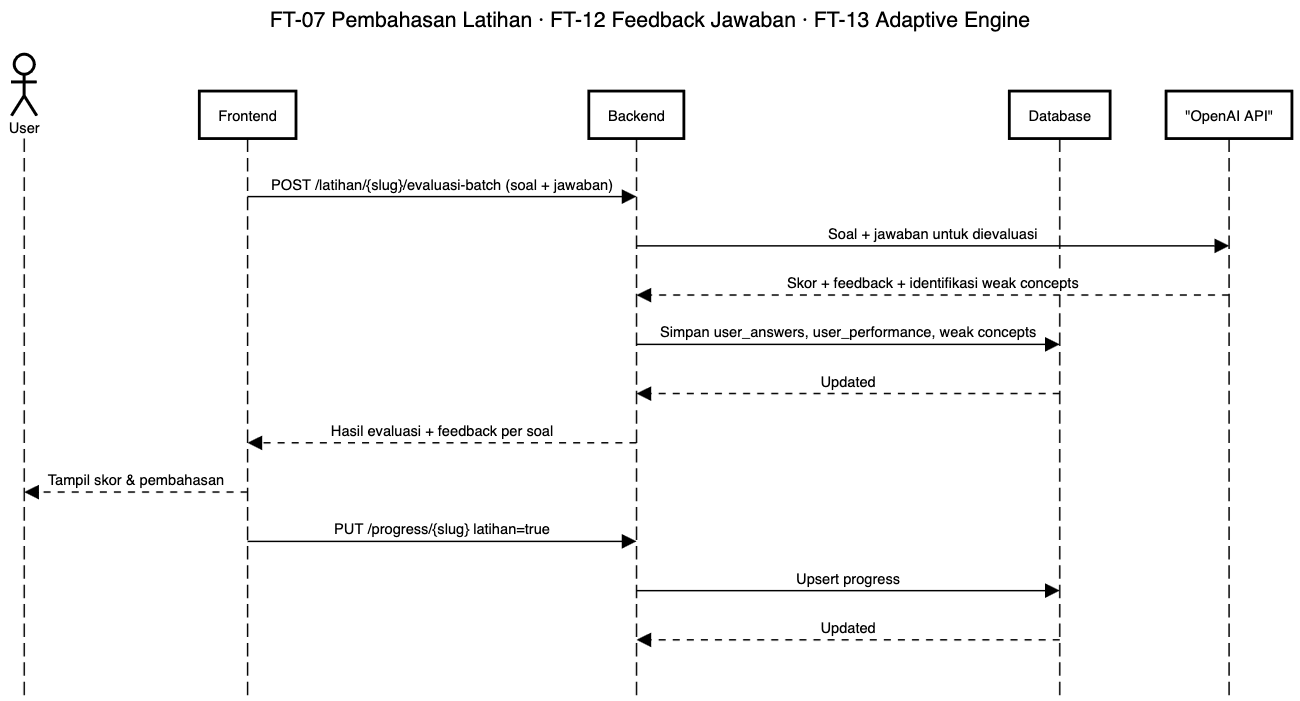
\includegraphics[width=0.9\textwidth]{images/FT-07-Pembahasan-Latihan-FT-12-Feedback-Jawaban-FT-13-Adaptive-Engine.png}
    \caption{\textit{Sequence Diagram} FT-07 Pembahasan Latihan, FT-12 \textit{Feedback} Jawaban, dan FT-13 \textit{Adaptive Engine}}
    \label{fig:sd-pembahasan}
\end{figure}

Diagram pada Gambar \ref{fig:sd-pembahasan} menggambarkan alur evaluasi jawaban dan pembaruan model adaptif. Setelah \textit{user} mengirim jawaban, \textit{frontend} meneruskan seluruh pasangan soal dan jawaban ke \textit{backend} melalui \texttt{POST /latihan/\{slug\}/evaluasi-batch}. \textit{Backend} mengirimkan data tersebut ke OpenAI API untuk dievaluasi, dan API mengembalikan skor, \textit{feedback} per soal, serta identifikasi \textit{weak concepts} baru. \textit{Backend} menyimpan hasil evaluasi — termasuk \texttt{user\_answers}, \texttt{user\_performance}, dan \textit{weak concepts} — ke \textit{database} untuk digunakan sebagai dasar adaptasi pada sesi berikutnya. \textit{Frontend} kemudian menampilkan skor dan pembahasan kepada \textit{user}, dan memperbarui progres dengan status \texttt{latihan=true}.

\begin{figure}[H]
    \centering
    \textbf{FT-08 Ringkasan Materi}\\[6pt]
    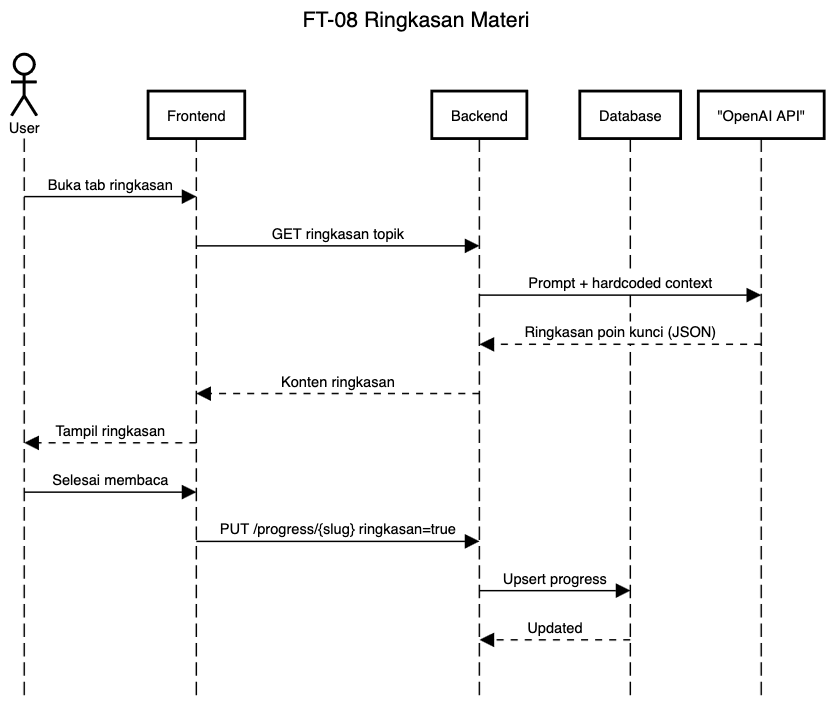
\includegraphics[width=0.9\textwidth]{images/FT-08-Ringkasan-Materi.png}
    \caption{\textit{Sequence Diagram} FT-08 Ringkasan Materi}
    \label{fig:sd-ringkasan}
\end{figure}

Diagram pada Gambar \ref{fig:sd-ringkasan} menggambarkan alur penampilan ringkasan materi di akhir sesi belajar. \textit{Frontend} mengirim permintaan \texttt{GET} ringkasan ke \textit{backend}, yang kemudian meneruskan \textit{prompt} beserta konteks materi ke OpenAI API. API menghasilkan ringkasan poin-poin kunci dalam format JSON. Setelah \textit{user} selesai membaca ringkasan, progres diperbarui dengan status \texttt{ringkasan=true}, menandakan bahwa \textit{user} telah menyelesaikan seluruh tahapan pembelajaran untuk topik tersebut.

\begin{figure}[H]
    \centering
    \textbf{FT-09 Progres Belajar + FT-13 \textit{Adaptive Engine}}\\[6pt]
    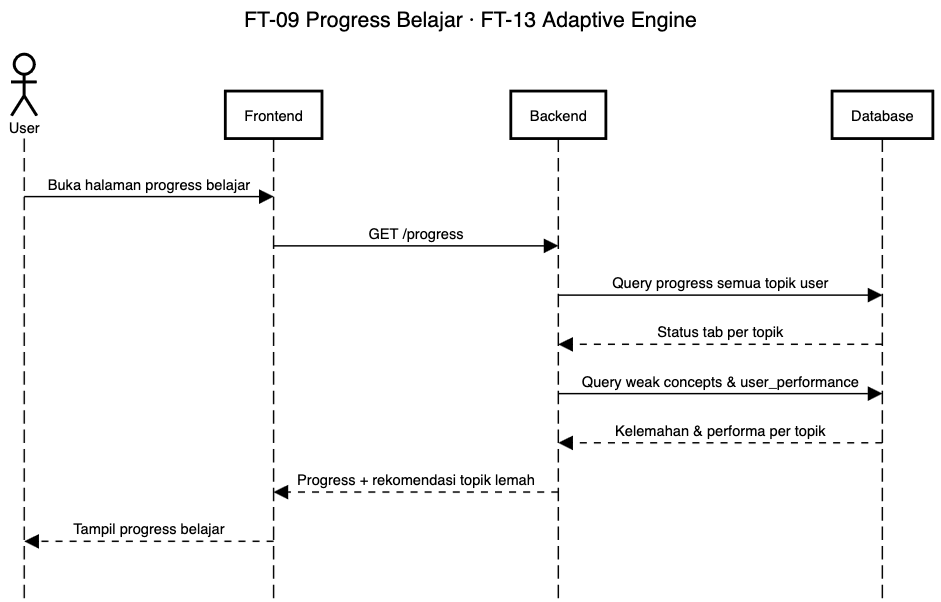
\includegraphics[width=0.9\textwidth]{images/FT-09-Progress-Belajar-FT-13-Adaptive-Engine.png}
    \caption{\textit{Sequence Diagram} FT-09 Progres Belajar dan FT-13 \textit{Adaptive Engine}}
    \label{fig:sd-progress}
\end{figure}

Diagram pada Gambar \ref{fig:sd-progress} menggambarkan alur penampilan halaman progres belajar yang terintegrasi dengan \textit{adaptive engine}. \textit{Frontend} meminta data melalui \texttt{GET /progress}, dan \textit{backend} melakukan dua \textit{query} ke \textit{database}: pertama untuk mengambil status tab seluruh topik, dan kedua untuk mengambil data \textit{weak concepts} serta performa \textit{user} per topik. \textit{Backend} menggabungkan kedua data tersebut dan mengembalikan informasi progres lengkap beserta rekomendasi topik yang perlu diperkuat. \textit{Frontend} menampilkan seluruh informasi tersebut kepada \textit{user} dalam satu halaman yang komprehensif.


\section{Perancangan \textit{Database}}

\subsection{Spesifikasi \textit{Platform Database}}

PostgreSQL dipilih sebagai sistem manajemen \textit{database} karena bersifat \textit{open source}, mendukung tipe data relasional yang kaya, serta memiliki ekosistem yang matang untuk pengembangan aplikasi web. Akses ke \textit{database} dilakukan melalui SQLAlchemy sebagai ORM (\textit{Object-Relational Mapper}) dengan \textit{driver} psycopg3, sehingga interaksi antara \textit{backend} Python dan \textit{database} dapat dilakukan secara efisien dan aman. Tabel \ref{tab:spek-db} menyajikan spesifikasi \textit{platform database} yang digunakan.

\begin{table}[H]
    \centering
    \caption{Spesifikasi \textit{Platform Database}}
    \label{tab:spek-db}
    \begin{tabular}{|p{4cm}|p{8cm}|}
    \hline
    \textbf{Aspek} & \textbf{Spesifikasi} \\
    \hline
    \textit{Database Engine} & PostgreSQL \\
    \hline
    \textit{Driver} & psycopg (psycopg3) \\
    \hline
    ORM & SQLAlchemy \\
    \hline
    Nama \textit{Database} & \texttt{asd\_learning\_db} \\
    \hline
    Port & 5432 (default) \\
    \hline
    \end{tabular}
\end{table}

\subsection{Desain Skema \textit{Database}}
\section{Perancangan \textit{Website}}
\subsection{Perancangan API}
\subsection{Perancangan Antarmuka}
Will be attached later
\subsection{Spesifikasi \textit{Hosting}}